\section{Decay Angles}
\label{sec:ana_angles}

Also the measurement of the decay angles has a finite precision and is affected by a non-trivial acceptance shape. Whereas resolution
effects in decay time directly affect the amplitude of the measured decay-time oscillation and, therefore, the estimates of the
CP-violation parameters, the effect of angular resolution are indirect and expected to be smaller. Because a convolution of the angular
functions in the decay model with a resolution function would be far from trivial, angular resolution is not included in the model of the
decay. However, resolution effects cannot be entirely neglected and do introduce systematic uncertainties in the final parameter estimates
(see Section~\ref{sec:result_syst}).

The acceptance as a function of decay angles is included in the decay model. It can either be modelled as a function or by so-called
\emph{normalization weights}, as will be described in Sections~\ref{subsec:ana_angles_param} and \ref{subsec:ana_angles_weights},
respectively. The shape of the acceptance function is determined from simulated decays, for which the observed angular distribution
including acceptance effects can be compared to the original distribution that was generated.

The shape of the angular acceptance function is shown in Figure~\ref{fig:angAcc}. The figure shows the acceptance function for each of
three angles, integrated over the two remaining angles. The data points are sums of simulated decays, weighted by the inverse of the PDF
that was used to generate the decays at each point in decay angles. This results in the ratio of the observed distribution including
acceptance effects and the generated distribution. The shape of this ratio in the decay angles is given by the shape of the angular
acceptance function. In essence this is also how the acceptance function for the decay model, represented by the blue line, is determined.

\begin{figure}[tbp]
  \centering
  \begin{subfigure}{0.49\textwidth}
    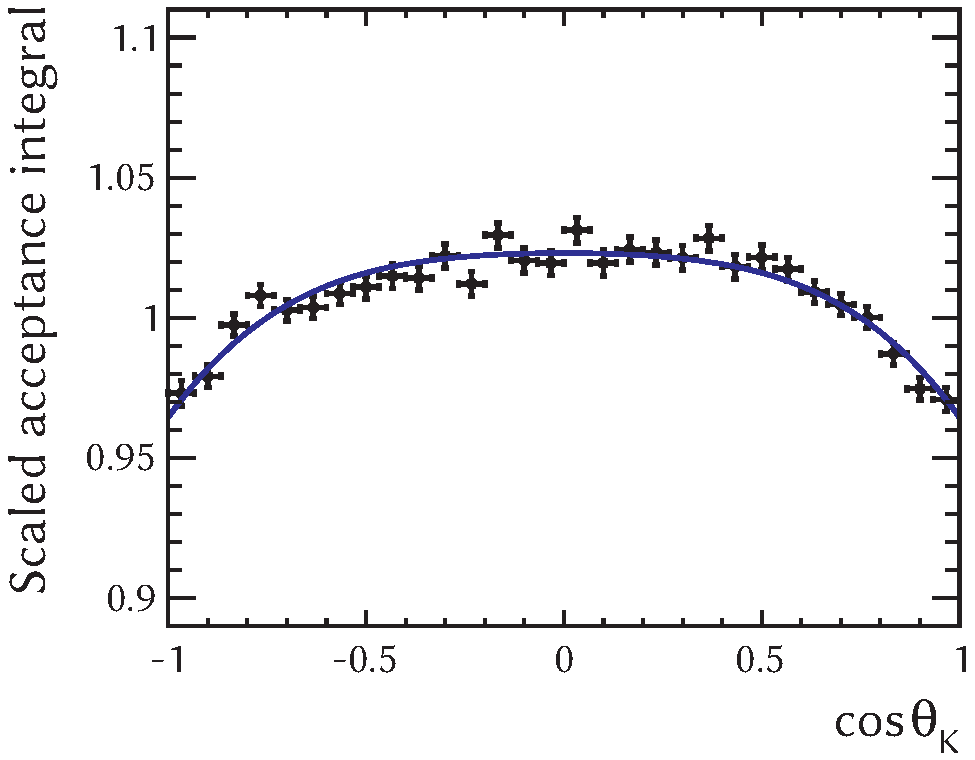
\includegraphics[width=\textwidth]{graphics/analysis/angAcc_ctk}
    \caption{}
    \label{fig:angAcc_ctk}
  \end{subfigure}%
  \hfill%
  \begin{subfigure}{0.49\textwidth}
    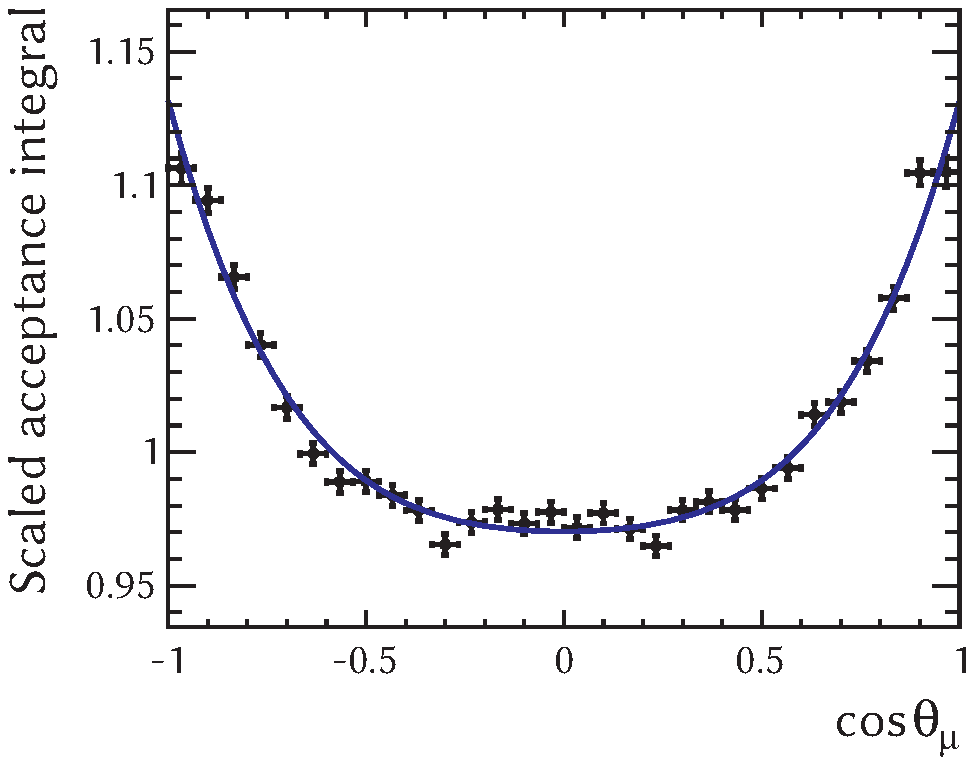
\includegraphics[width=\textwidth]{graphics/analysis/angAcc_ctl}
    \caption{}
    \label{fig:angAcc_ctl}
  \end{subfigure}

  \vspace*{0.02\textwidth}
  \begin{subfigure}{0.49\textwidth}
    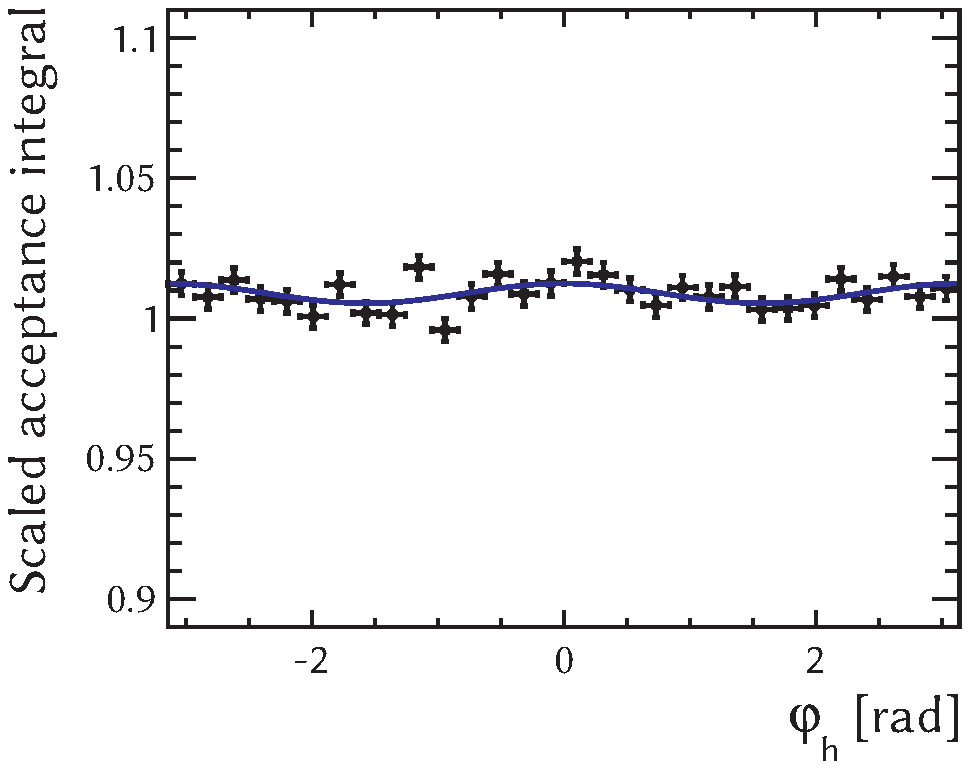
\includegraphics[width=\textwidth]{graphics/analysis/angAcc_phi}
    \caption{}
    \label{fig:angAcc_phi}
  \end{subfigure}
  \caption{Shape of the acceptance function in each of the three decay angles: (a) $\cthetaK$, (b) $\cthetal$, (c) $\phihel$.
           The angular acceptance function is integrated over the two remaining angles in each of the figures.
           The blue line represents a parameterization of the function in terms of Legendre polynomials for $\cthetaK$
           and real-valued spherical harmonics for $\cthetal$ and $\phihel$.
           The data points are obtained by a sum over simulated decays, which are weighted by the value of the PDF that was used to
           generate the decays at each point in decay angles.
           Notice that the vertical scale of these figures does not start at zero.}
  \label{fig:angAcc}
\end{figure}

Following the above reasoning, the observed angular shape of simulated decays, after detector simulation and selection, can be expressed as
the generated shape multiplied by the acceptance function. Normalizing these two shapes to obtain the observed and generated PDFs, the
ratio of the two distributions can be written as
\begin{equation}
  \begin{aligned}
    \frac{P^\text{obs}(\Omega|t)}{P^\text{gen}(\Omega|t)}
        &= \frac{\effta\, p(t,\Omega)}{\int\ud\Omega\; \effta\, p(t,\Omega)}\; \frac{\int\ud\Omega\; p(t,\Omega)}{p(t,\Omega)}\\
         = &\frac{\effta\, \int\ud\Omega\; p(t,\Omega)}{\int\ud\Omega\; \effta\, p(t,\Omega)}
         = \frac{\effta}{\int\ud\Omega\; \effta\, P^\text{gen}(\Omega|t)}
         = \frac{\effta}{\meff(t)}\\
        \effta &= \meff(t)\; \frac{P^\text{obs}(\Omega|t)}{P^\text{gen}(\Omega|t)} \ ,
  \end{aligned}
  \label{eq:angAccPDFRatio}
\end{equation}
where $P^\text{obs}$ is the observed PDF, $P^\text{gen}$ the generated PDF, $p$ the function of time and angles from which the PDFs are
built, and $\eff$ the time and angular acceptance function. Both angular PDFs are conditional on decay time. The angular mean of the
acceptance function, which depends on decay time, is given by
\begin{equation}
  \meff(t) \equiv \int\ud\Omega\, \effta\, P^\text{gen}(\Omega|t)\ .
\end{equation}

Assuming the time and angular acceptance functions factorize, that is $\effta = \efft \times \effa$, the mean acceptance can be expressed
as
\begin{equation}
  \meff(t) = \efft \times \int\ud\Omega\, \effa\, P^\text{gen}(\Omega|t)
           = \efft \times \meffa(t) \ .
\end{equation}
Inserting this expression into the last line of Equation~\ref{eq:angAccPDFRatio} yields for the acceptance function
\begin{equation}
  \effta = \efft \times \meffa(t)\; \frac{P^\text{obs}(\Omega|t)}{P^\text{gen}(\Omega|t)}\ ,
\end{equation}
which means that the angular acceptance function is given by
\begin{equation}
  \label{eq:angAcc}
  \effa = \meffa(t)\; \frac{P^\text{obs}(\Omega|t)}{P^\text{gen}(\Omega|t)}\ .
\end{equation}
The factor $\meffa(t)$ is the mean of the angular acceptance function, which generally depends on decay time. Since only the shape of the
angular acceptance function is relevant in this model, it is not required to determine the value of this angular constant factor. The ratio
of the observed and generated PDFs suffices to determine the shape of the function in the decay angles.


%%%%%%%%%%%%%%%%%%%%%%%%%%%%%%%%%%%%%%%%
\subsection{Acceptance Parameterization}
\label{subsec:ana_angles_param}
%%%%%%%%%%%%%%%%%%%%%%%%%%%%%%%%%%%%%%%%

The function $\effa$ is represented in Figure~\ref{fig:angAcc} by the blue line. For this figure, it is parameterized in terms of Legendre
polynomials and real-valued spherical harmonics, $\Lp{j}(\cthetaK)\,\rsph{l}{m}(\cthetal,\phihel)$ (see also
Section~\ref{sec:angularDecay_squareAmp}, Equations~\ref{eq:PYdef} and \ref{eq:realYdef}). These functions form an orthogonal basis of
functions of the three decay angles.

In principle an arbitrary function is expressed as an infinite sum of basis functions, but in practice the relatively uniform acceptance
function can be described by a limited number of contributions. The function $\Lp{0}\,\rsph{0}{0}$ is a constant and would be the only
contribution for a truly uniform acceptance function. A few higher-order functions up to $j$\texteq4, $l$\texteq4, and $m$\texteq2 are
included to describe the shape shown in Figure~\ref{fig:angAcc}. Even higher orders represent faster changes in the acceptance function and
can be omitted for this slowly-changing shape.

The coefficients of the basis functions, which specify the shape of the acceptance function, are determined from the simulated
\BstoJpsiKK{} decays that were used for Figure~\ref{fig:angAcc}. Expressing the acceptance function as
\begin{equation}
  \effa = \sum_{j,l,m} c_{jlm}\,b_{jlm}(\Omega)\ ,
\end{equation}
the coefficients are defined as
\begin{equation}
  \label{eq:angEffCoefDef}
  c_{jlm} \equiv (j+\tfrac{1}{2}) \int\ud\Omega\,b_{jlm}(\Omega)\,\effa\ ,
\end{equation}
where $b_{jlm}$ is a basis function and $c_{jlm}$ the corresponding coefficient. The normalization factor $j+\tfrac{1}{2}$ arises from the
fact that Legendre polynomials are orthogonal, but not orthonormal:
\begin{equation}
  \int\ud\cthetaK\,\Lp{j}(\cthetaK)\cdot\Lp{j}(\cthetaK) = \frac{1}{j+\tfrac{1}{2}}\ .
\end{equation}

The integral in Equation~\ref{eq:angEffCoefDef} is calculated by means of Monte Carlo integration, using the simulated decays. A constant
is defined to absorb the factor $\meffa(t)$ in Equation~\ref{eq:angAcc}:
\begin{equation}
  \label{eq:angEffConst}
  E_a \equiv \left[ \int\ud t\, \frac{P^\text{obs}(t)}{\meffa(t)} \right]^{-1}\ .
\end{equation}
Notice that $E_a$ reduces to the mean angular acceptance, $\meffa$, if the PDFs for time and angles factorize,
$P^\text{gen}(t,\Omega)$\texteq$P^\text{gen}(t)$\texttimes$P^\text{gen}(\Omega)$. In this case $P^\text{gen}(\Omega|t)$ is equal to
$P^\text{gen}(\Omega)$ and $\meffa$ is independent of time and the integral in Equation~\ref{eq:angEffConst} evaluates to $\meffa^{-1}$.

With the constant $E_a$ and the definition of the angular acceptance in Equation~\ref{eq:angAcc}, the coefficients of
Equation~\ref{eq:angEffCoefDef} can be expressed as
\begin{equation}
  \label{eq:angAccInt}
  \begin{split}
    \tfrac{1}{E_a}\, c_{jlm} &= \int\ud t\, \frac{P^\text{obs}(t)}{\meffa(t)}
                                \cdot (j+\tfrac{1}{2}) \int\ud\Omega\,b_{jlm}(\Omega)\, \effa \\
                             &= (j+\tfrac{1}{2}) \int\ud t\, \ud\Omega\; \frac{P^\text{obs}(t)}{\meffa(t)}\,
                                b_{jlm}(\Omega)\, \meffa(t)\, \frac{P^\text{obs}(\Omega|t)}{P^\text{gen}(\Omega|t)} \\
                             &= (j+\tfrac{1}{2}) \int\ud t\, \ud\Omega\; P^\text{obs}(t,\Omega)\,
                                \frac{b_{jlm}(\Omega)}{P^\text{gen}(\Omega|t)} \ .
  \end{split}
\end{equation}
The value of this integral is estimated with a sum over simulated decays:
\begin{equation}
  E\left( \tfrac{1}{E_a}\, c_{jlm} \right)
      = (j + \tfrac{1}{2})\, \frac{1}{N^\text{obs}}\, \sum_{e=1}^{N^\text{obs}}\frac{b_{jlm}(\Omega_e)}{P^\text{gen}(\Omega_e|t_e)}
  \label{eq:angEffCoefEst}
\end{equation}
Since the ``mean acceptance'' is a constant equal for all coefficients, this factor can be ignored for the shape of the acceptance
function. The values of the coefficients that were used for the function in Figure~\ref{fig:angAcc} are specified in
Table~\ref{tab:angEffCoefs}. Note that, although not shown in the table, there are correlations between these estimates.
\begin{table}[htbp]
  \centering
  \caption{Values of the coefficients of the angular acceptance function that were used for the function shown in Figure~\ref{fig:angAcc},
           obtained from simulated \BstoJpsiKK{} decays.
           The specified values are estimates of the quantity $\tfrac{1}{E_a}\, c_{jlm}$ (Equation~\ref{eq:angEffCoefEst}).}
  \label{tab:angEffCoefs}
  \begin{tabular}{ccc}
    \hline
    coefficient ($jlm$)  &  value  &  statistical uncertainty  \\
    \hline
    000  &   3.5767  &  0.0011  \\
    020  &  +0.1535  &  0.0030  \\
    040  &  +0.0305  &  0.0031  \\
    022  &  +0.0096  &  0.0026  \\
    200  &  -0.125   &  0.006   \\
    400  &  -0.033   &  0.008   \\
    \hline
  \end{tabular}
\end{table}

For a uniform acceptance function, $\effa$\texteq$\meffa$\texteq constant, and Equation~\ref{eq:angAccInt} reduces to
\begin{equation}
  \tfrac{1}{E_a}\, c_{jlm} = (j+\tfrac{1}{2}) \int\ud\Omega\,b_{jlm}(\Omega)\ .
\end{equation}
This integral is only non-zero for $j$\texteq$l$\texteq$m$\texteq0, for which $\tfrac{1}{E_a}\,c_{000}$\texteq2$\sqrt{\pi}$\textapprox3.54.
Table~\ref{tab:angEffCoefs} shows that the acceptance function is not too far from being uniform.


%%%%%%%%%%%%%%%%%%%%%%%%%%%%%%%%%
\subsection{Acceptance Normalization Weights}
\label{subsec:ana_angles_weights}
%%%%%%%%%%%%%%%%%%%%%%%%%%%%%%%%%

In principle the parameterization of the acceptance function in terms of Legendre polynomials and spherical harmonics could be used to
describe the acceptance function in the PDF for the time and angular fit. However, this would require criteria that specify which set of
basis functions to include in the description and a study of the effect of not including functions that are not in this set. A slightly
different approach circumvents this problem and includes all relevant acceptance information.

Using the notation of Equation~\ref{eq:angAccPDFRatio}, the PDF including acceptance effects is given by
\begin{equation}
  \label{eq:obsPDF}
  P^\text{obs}(t,\Omega) = \frac{\effta\, p(t,\Omega)}{\int\ud t\, \ud\Omega\; \effta\, p(t,\Omega)}
\end{equation}
Assuming the time and angular acceptance functions factorize and writing the function $p(t,\Omega)$ in the normalization integral as a sum
of angular terms (see Sections~\ref{sec:pheno_angles} and \ref{sec:pheno_equations}), the PDF can be expressed as
\begin{equation}
  \label{eq:obsPDFNormSum}
  P^\text{obs}(t,\Omega) = \efft\,\effa\, \frac{p(t,\Omega)}{\sum_k \int\ud t\, \efft f_{t,k}(t) \int\ud\Omega\, \effa f_{a,k}(\Omega)}\ ,
\end{equation}
where $f_{t,k}(t)$ and $f_{a,k}(\Omega)$ are the time and angular functions of a term $k$ in the differential decay rate, respectively (see
Equation~\ref{eq:timeqfDep} and Table~\ref{tab:angDist}).

If the angular acceptance function does not contain any free parameters, the factor $\effa$ in Equation~\ref{eq:obsPDFNormSum} becomes a
constant term in the minimization of the NLL (see also Section~\ref{sec:ana_fit}) and can be ignored. The angular acceptance function then
only remains in the normalization integral $\int\ud\Omega\, \effa f_{a,k}(\Omega)$. This integral is very similar to the integral in
Equation~\ref{eq:angEffCoefDef} and can be estimated in the same way (Equations~\ref{eq:angAccInt} and \ref{eq:angEffCoefEst}).

This procedure leads to the definition of \emph{normalization weights}, which were first described in \cite{duPree:2010}. The weights are
determined for each term in the differential decay rate and are defined by
\begin{equation}
  \label{eq:angNormWeightDef}
  \xi_k \equiv \int\ud\Omega\, \effa f_{a,k}(\Omega)\ ,
\end{equation}
with a corresponding estimate from simulated events
\begin{equation}
  \label{eq:angNormWeightEst}
  E\left( \tfrac{1}{E_a}\, \xi_k \right)
      = \frac{1}{N^\text{obs}}\, \sum_{e=1}^{N^\text{obs}}\frac{f_{a,k}(\Omega_e)}{P^\text{gen}(\Omega_e|t_e)}\ .
\end{equation}
The estimated values of the normalization weights are given in Table~\ref{tab:angNormWeights}. The largest correlations between these
estimates are found between the ``00'' weight and the ``$\parallel\parallel$'' and ``$\perp\perp$'' weights; -68\% and -69\%, respectively.
\begin{table}[htbp]
  \centering
  \caption{Values of the normalization weights of the angular acceptance function.
           The specified values are estimates of the quantity $\tfrac{1}{E_a}\, \xi_k$ (Equation~\ref{eq:angNormWeightEst}).}
  \label{tab:angNormWeights}
  \begin{tabular}{ccc}
    \hline
    weight ($k$)  &  value  &  statistical uncertainty  \\
    \hline
    00                    &  0.9744   &  0.0005  \\
    $\parallel\parallel$  &  1.0245   &  0.0006  \\
    $\perp\perp$          &  1.0263   &  0.0006  \\
    0$\parallel$          &  +0.0001  &  0.0005  \\
    0$\perp$              &  -0.0003  &  0.0004  \\
    $\parallel\perp$      &  -0.0006  &  0.0007  \\
    SS                    &  0.9896   &  0.0004  \\
    0S                    &  +0.0007  &  0.0014  \\
    $\parallel$S          &  +0.0007  &  0.0006  \\
    $\perp$S              &  +0.0003  &  0.0006  \\
    \hline
  \end{tabular}
\end{table}

For a uniform angular acceptance function, the expression for the acceptance weights reduces to
\begin{equation}
  \tfrac{1}{E_a}\, \xi_k = \int\ud\Omega\,f_{a,k}(\Omega)\ .
\end{equation}
This integral evaluates to 1 for the ``diagonal'' terms ``00'', ``$\parallel\parallel$'', ``$\perp\perp$'', and ``SS'' and vanishes for the
remaining interference terms. The values of the acceptance weights confirm that the acceptance function is close to being uniform.

Since the full set of basis-function coefficients contains all the information on the angular acceptance function, the acceptance weights
can be expressed in terms of the coefficients. Because the weights only contain the information that is required for the PDF normalization
integral, the set of weights does not completely specify the acceptance function and the transformation from weights to coefficients is
ambiguous. That is, there is an infinitely large set of acceptance functions that yields a given set of normalization weights.

Expressions for the acceptance weights in terms of basis coefficients are derived by expressing the decay-rate functions $f_{a,k}$ in terms
of basis functions. The integral of Equation~\ref{eq:angNormWeightDef} can then be expressed as a sum of the basis-function integrals in
Equation~\ref{eq:angEffCoefDef}. The resulting expressions for the acceptance weights are given by
\begin{equation}
  \label{eq:angCoefToWeight}
  \begin{alignedat}{2}
    2\sqrt{\pi}\; &\xi_{\text{00}} &
      &= c_{000} - \tfrac{1}{\sqrt{5}} c_{020} + \tfrac{2}{5} c_{200} - \tfrac{2}{5\sqrt{5}} c_{220} \\
    2\sqrt{\pi}\; &\xi_{\parallel\parallel} &
      &= \tfrac{1}{2}\,(2 c_{000} + \tfrac{1}{\sqrt{5}} c_{020} - \sqrt{\tfrac{3}{5}} c_{022} - \tfrac{2}{5} c_{200}
         - \tfrac{1}{5\sqrt{5}} c_{220} + \tfrac{1}{5}\sqrt{\tfrac{3}{5}} c_{222}) \\
    2\sqrt{\pi}\; &\xi_{\perp\perp} &
      &= \tfrac{1}{2}\,(2 c_{000} + \tfrac{1}{\sqrt{5}} c_{020} + \sqrt{\tfrac{3}{5}} c_{022} - \tfrac{2}{5} c_{200}
         - \tfrac{1}{5\sqrt{5}} c_{220} - \tfrac{1}{5}\sqrt{\tfrac{3}{5}} c_{222}) \\
    2\sqrt{\pi}\; &\xi_{\text{0}\parallel} &
      &= -\tfrac{3}{32}\sqrt{\tfrac{6}{5}}\pi\, (c_{121} - \tfrac{1}{4} c_{321} - \tfrac{5}{128} c_{521} - \ldots) \\
    2\sqrt{\pi}\; &\xi_{\text{0}\perp} &
      &= +\tfrac{3}{32}\sqrt{\tfrac{6}{5}}\pi\, (c_{12\,-1} - \tfrac{1}{4} c_{32\,-1} - \tfrac{5}{128} c_{52\,-1} - \ldots) \\
    2\sqrt{\pi}\; &\xi_{\parallel\perp} &
      &= \sqrt{\tfrac{3}{5}}\, (c_{02\,-2} - \tfrac{1}{5} c_{22\,-2}) \\
    2\sqrt{\pi}\; &\xi_{\text{SS}} &
      &= c_{000} - \tfrac{1}{\sqrt{5}}\,c_{020} \\
    2\sqrt{\pi}\; &\xi_{\text{0S}} &
      &= \tfrac{2}{\sqrt{3}}\, (c_{100} - \tfrac{1}{\sqrt{5}} c_{120}) \\
    2\sqrt{\pi}\; &\xi_{\parallel\text{S}} &
      &= -\tfrac{3}{8}\sqrt{\tfrac{2}{5}}\pi\, (c_{021} - \tfrac{1}{8} c_{221} - \tfrac{1}{64} c_{421} - \ldots) \\
    2\sqrt{\pi}\; &\xi_{\perp\text{S}} &
      &= -\tfrac{3}{8}\sqrt{\tfrac{2}{5}}\pi\, (c_{02\,-1} - \tfrac{1}{8} c_{22\,-1} - \tfrac{1}{64} c_{42\,-1} - \ldots) \ .
  \end{alignedat}
\end{equation}
